\section{Conics: classification, parametrization, and metric properties}
\label{sec:conics}

This chapter treats the conic and quadric topics linked directly from the
analytic-geometry article. All classification inputs are rational numbers.
Consequently every test of a coefficient, determinant, or discriminant is a
decidable test on integer codes. A statement about a point with represented
real coordinates denotes the fixed-family, precision-indexed interpretation
specified in the foundations chapter. In particular, a real denominator is
used only with a positive rational lower bound on its absolute value. Square
roots below are the nonnegative roots, constructed by bounded dyadic search.
Classification of rational coefficients does not purport to decide the sign
of an arbitrary represented real number.

\subsection{Matrices and a complete classification algorithm}

\begin{figure}[htbp]
\centering
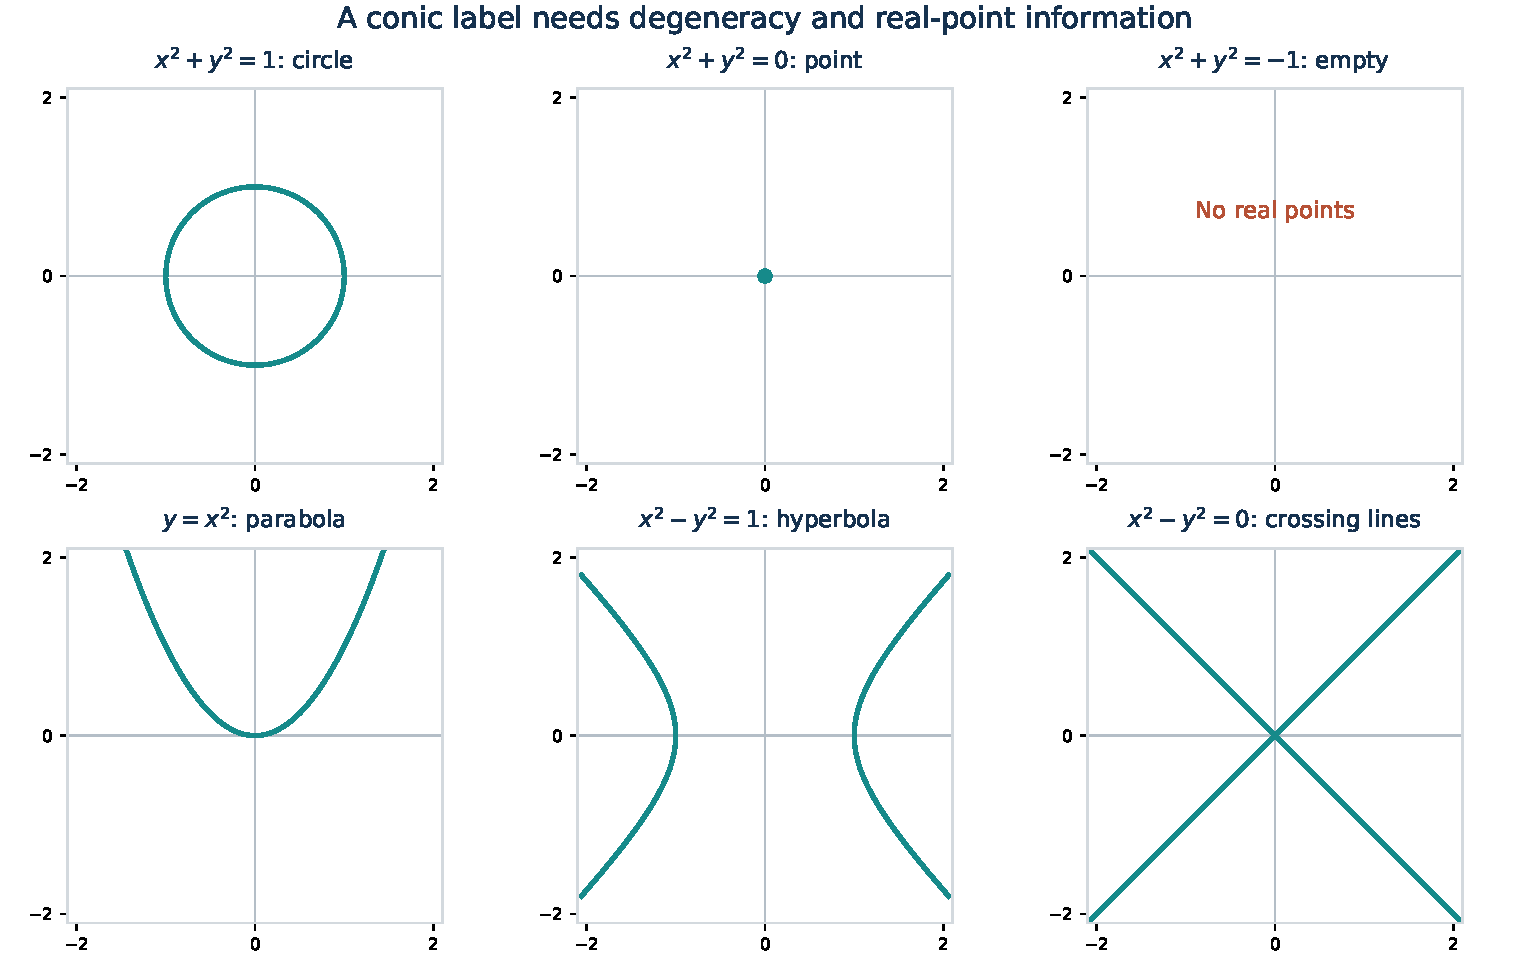
\includegraphics[width=.94\linewidth]{figures/conic_loci.pdf}
\caption{Real loci of explicit rational quadratics. The first row has the
same discriminant $-4$ throughout; the constant term distinguishes a circle,
a point, and an empty locus. The proof of classification uses exact rational
tests, not the plots.}
\end{figure}

Put
\[
 q(x,y)=Ax^2+Bxy+Cy^2+Dx+Ey+F,\qquad
 S=\begin{pmatrix}A&B/2\\B/2&C\end{pmatrix},\quad
 \ell=\binom D E,
\]
and put
\[
 H=\begin{pmatrix}A&B/2&D/2\\B/2&C&E/2\\D/2&E/2&F\end{pmatrix}.
\]
Thus, with $X=(x,y)^T$ and $Z=(x,y,z)^T$,
$q(X)=X^TSX+\ell^TX+F$ and
$q_h(Z)=Z^THZ$ is its homogenization. Homogeneous coordinates mean nonzero
triples modulo multiplication by a nonzero scalar; only this explicitly
described equivalence relation is needed here.

\begin{proposition}[Scaling and coordinate covariance]\label{con:covariance}
Multiplication of all coefficients by a nonzero rational scalar preserves
the zero locus. Under an invertible rational affine substitution $X=MU+t$,
the new quadratic matrix is $M^TSM$. The homogeneous matrix is $T^THT$, where
$T=\left(\begin{smallmatrix}M&t\\0&1\end{smallmatrix}\right)$.
In particular, the substitution and its explicitly computed inverse give
mutually inverse maps of the two zero loci.
\end{proposition}
\begin{proof}
For a nonzero scalar $s$, $sq(X)=0$ implies $q(X)=0$ by multiplication by
$1/s$, and the converse is immediate. Expanding the substitution gives
\[
 q(MU+t)=U^TM^TSMU+(2t^TSM+\ell^TM)U+q(t).
\]
This proves the affine formula, while $(TZ)^TH(TZ)=Z^T(T^THT)Z$ proves
the homogeneous formula. The inverse is $U=M^{-1}(X-t)$, with
$M^{-1}=\operatorname{adj}(M)/\det M$. These are rational operations on a
fixed number of coordinates, with the guard $\det M\ne0$ checked before
division.
\end{proof}

\begin{theorem}[Discriminant and projective singularity]\label{con:invariants}
Let $\Delta=B^2-4AC$. Under the preceding affine substitution,
$\Delta'=(\det M)^2\Delta$. A projective conic is singular, in the sense
that some nonzero homogeneous vector $Z$ satisfies $HZ=0$, if and only if
$\det H=0$. For rational coefficients, existence of such a singular vector
is decided and witnessed by finite rational elimination. When $\det H\ne0$,
no entire affine line is contained in the conic.
\end{theorem}
\begin{proof}
The equality $\Delta=-4\det S$ and determinant multiplication give the
first formula. If $HZ=0$ and $Z\ne0$, an inverse for $H$ would force $Z=0$;
thus $\det H\ne0$ is impossible. Conversely, if the determinant vanishes,
ordinary elimination in three columns chooses the first nonzero rational
pivot when one exists. At least one column is free. Set its free variable
to $1$, the other free variables to $0$, and back-substitute. This produces
a nonzero rational null vector. It also satisfies $q_h(Z)=Z^THZ=0$;
the homogeneous partial derivatives are the coordinates of $2HZ$.

For the last assertion, use an invertible rational affine change sending
a proposed rational affine line to $v=0$. Vanishing identically on it
forces the constant, $u$, and $u^2$ coefficients to vanish. The transformed
polynomial is therefore $v(\alpha u+\beta v+\gamma)$. Its homogeneous
matrix is a sum of two matrices of rank at most one, so has determinant
zero, a fact also obtained by expanding its $3$ by $3$ determinant.
For a line given by represented-real data with certified invertible
coordinate change the same identity applies. Thus a nonsingular conic
cannot contain such a line.
\end{proof}

\begin{lemma}[Rational completion of squares]\label{con:completion}
If $A\ne0$, set
\[
 u=x+\frac{B}{2A}y+\frac{D}{2A},\quad
 K=C-\frac{B^2}{4A},\quad
 L=E-\frac{BD}{2A},\quad M_0=F-\frac{D^2}{4A}.
\]
Then $q=Au^2+Ky^2+Ly+M_0$. If also $K\ne0$, setting
$v=y+L/(2K)$ and $J=M_0-L^2/(4K)$ gives $q=Au^2+Kv^2+J$.
Every nonzero binary quadratic part can be brought to the case $A\ne0$
by an explicitly invertible rational linear change.
\end{lemma}
\begin{proof}
Expanding $Au^2$ gives the original $Ax^2+Bxy+Dx$ and adds
$B^2y^2/(4A)+BDy/(2A)+D^2/(4A)$. The displayed values of $K,L,M_0$
subtract exactly those three additions. The second completion follows
by expanding $K(y+L/(2K))^2$.
If $A=0$ and $C\ne0$, exchange $x$ and $y$. If $A=C=0$ but $B\ne0$,
put $x=r+s$, $y=r-s$; then $Bxy=B r^2-Bs^2$ and the change has
determinant $-2$. These exhaust the nonzero cases by decidable rational
tests. The displayed transformations have explicit rational inverses.
\end{proof}

\begin{theorem}[Exhaustive real-locus classification for rational conics]
\label{con:classification}
There is a primitive recursive procedure returning an invertible rational
affine change and one of the following descriptions. Subsequent positive
rescalings by represented square roots identify the named standard shapes.
For crossing components, the constructive output is their factored
equation; membership in a chosen component for arbitrary represented-real
points is asserted only with a branch certificate or separation from the
crossing. The ordinary shape names in the table carry this qualification.
\begin{center}
\begin{tabular}{p{.27\linewidth}p{.64\linewidth}}
Normal equation and guard & Real zero locus\\\hline
$Au^2+Kv^2=-J$, $AK>0$ & An ellipse if $-J/A>0$; one point if $J=0$;
empty if $-J/A<0$.\\
$Au^2+Kv^2=-J$, $AK<0$ & A hyperbola if $J\ne0$; two intersecting lines
if $J=0$.\\
$Au^2+Ly+M_0=0$, $L\ne0$ & A parabola.\\
$Au^2+M_0=0$ & Two parallel lines if $-M_0/A>0$; one repeated line if
$M_0=0$; empty if $-M_0/A<0$.\\
$Dx+Ey+F=0$ & A line if $(D,E)\ne(0,0)$; the whole plane if $D=E=F=0$;
empty otherwise.
\end{tabular}
\end{center}
Here $A\ne0$ in the first four rows. In the nondegenerate, nonempty cases,
$\Delta<0$, $\Delta=0$, and $\Delta>0$ distinguish ellipse, parabola, and
hyperbola respectively. The negative-discriminant test alone does not
assert nonemptiness.
\end{theorem}
\begin{proof}
Apply Lemma~\ref{con:completion}. If $K\ne0$ the equation is diagonal.
When $A,K$ have the same sign, divide by $A$; the left side is a sum
of two nonnegative squares with positive coefficients. A negative right
side is impossible, a zero right side forces both coordinates to vanish,
and a positive right side gives a rescaled unit circle. More explicitly,
if $R=-J/A>0$, write $u=\sqrt R\,U$ and
$v=\sqrt{R A/K}\,V$ to obtain $U^2+V^2=1$.

When $AK<0$ and $J\ne0$, multiply the equation by the sign of $-J$,
divide by $|J|$, and rescale the two coordinates by positive square roots.
One obtains $U^2-V^2=1$, after exchanging coordinates if necessary.
If $J=0$, the identity
$u^2-(-K/A)v^2=(u-\sqrt{-K/A}\,v)(u+\sqrt{-K/A}\,v)$
gives the two lines. The union statement has a constructive meaning:
for an arbitrary represented-real point one has the product identity,
and membership in a particular line needs a supplied branch, or positive
separation from their intersection. There is no unguarded decision of
which line contains a point at their crossing.

When $K=0$ but $L\ne0$, solve
$y=-Au^2/L-M_0/L$, an invertible affine image of a parabola. If $K=L=0$,
the equation reduces to $u^2=-M_0/A$ and gives the stated alternatives.
For a positive right side the roots have a positive separation, so their
branches can be chosen from a sufficiently accurate rational observation.
The linear case is solved by choosing a nonzero coefficient.

All branches here test rational data and the number of elimination steps
is fixed. In the diagonal rank-two case, $\Delta=-4AK$ up to a positive
square factor; in rank one it is zero. The parabola row has $L\ne0$.
This proves the final classification with the necessary degeneracy and
nonemptiness qualifications. In particular, $x^2+y^2+1=0$ is an explicit
empty negative-discriminant example.
\end{proof}

\begin{theorem}[Constructive principal axes, circles, and rectangular hyperbolas]
\label{con:axes}
For a rational symmetric matrix $S$, an orthonormal eigenbasis can be
constructed by rational operations and nonnegative square roots. Its
eigenvalues are
\[
 \lambda_\pm=\frac{A+C\pm\sqrt{(A-C)^2+B^2}}2.
\]
For a nonempty nondegenerate ellipse, the curve is a circle precisely
when $A=C$ and $B=0$. For a nondegenerate hyperbola its two asymptotic
directions are perpendicular precisely when $A+C=0$.
\end{theorem}
\begin{proof}
If $B=0$, the coordinate axes already form an eigenbasis. If $B\ne0$,
take $v=(B,2(\lambda_+-A))$. The characteristic equation
$(\lambda-A)(\lambda-C)-B^2/4=0$ verifies $Sv=\lambda_+v$.
The vector $v$ is nonzero with $\|v\|\ge |B|$; thus normalization has
a rational lower bound on its denominator. Its perpendicular
$w=(-v_2,v_1)$ has eigenvalue $\lambda_-$, because symmetry makes $Sw$
orthogonal to $v$ and its coefficient is the trace minus $\lambda_+$.
Normalizing $v,w$ gives the promised rotation. Translation to the center
then gives the usual principal-axis equation when $\det S\ne0$.

The two ellipse semiaxes are equal exactly when the two eigenvalues are
equal. Their squared difference is $(A-C)^2+B^2$, which vanishes exactly
when $A=C$ and $B=0$. For a hyperbola, after multiplying the equation
by $-1$ if needed, the diagonal quadratic part has coefficients
$\alpha>0$ and $-\beta<0$. Its asymptotic directions can be taken as
$(\sqrt\beta,\sqrt\alpha)$ and $(\sqrt\beta,-\sqrt\alpha)$.
Their dot product is $\beta-\alpha$, zero exactly when the trace
$\alpha-\beta$ vanishes. Orthogonal changes preserve dot products and
the original trace is $A+C$.
\end{proof}

\subsection{Intersections and rational parametrizations}

\begin{theorem}[Complete quadratic solver with degeneracies]\label{con:roots}
For rational $a,b,c$, the real solutions of $at^2+bt+c=0$ are determined
by a primitive recursive case distinction. If $a\ne0$, put
$\delta=b^2-4ac$. There are no roots for $\delta<0$, the single root
$-b/(2a)$ for $\delta=0$, and the two distinct represented roots
\[
 t_\pm=\frac{-b\pm\sqrt\delta}{2a}
\]
for $\delta>0$. In the latter case
$t_++t_-=-b/a$ and $t_+t_-=c/a$.
If $a=0\ne b$ the only root is $-c/b$. If $a=b=0$, there are all
parameters or none according as $c=0$ or $c\ne0$.
\end{theorem}
\begin{proof}
For $a\ne0$, direct expansion yields
\[
 4a(at^2+bt+c)=(2at+b)^2-\delta.
\]
A square cannot be negative; a zero square has zero base. For $\delta>0$,
let $r=\sqrt\delta$. The two displayed values satisfy the equation,
and their difference is $r/a\ne0$. Conversely, a root has
$(2at+b)^2=r^2$. Put $h=\min(1,\delta)$, so $r\ge h>0$, and obtain
a rational approximation $s_0$ to $s=2at+b$ with error at most $h/4$.
If $s_0\ge0$, then $s+r\ge3h/4$; cancel that guarded factor in
$(s-r)(s+r)=0$ to obtain $s=r$. If $s_0<0$, then $r-s\ge3h/4$;
cancel it instead to obtain $s=-r$. Thus this completeness assertion
uses positive separation and one rational test, not real trichotomy.
Adding and multiplying the formulas
proves the two Vieta identities. The remaining cases are linear
identities with rational zero tests.
\end{proof}

\begin{corollary}[Line--conic intersection]\label{con:line-intersection}
For a rational conic and a rational line $P+tv$ with $v\ne0$, intersections
are obtained by the preceding solver with
\[
 \alpha=v^TSv,\qquad \beta=2P^TSv+\ell^Tv,\qquad \gamma=q(P).
\]
A line is contained in the conic exactly when $\alpha=\beta=\gamma=0$.
Otherwise it has at most two distinct intersections, and the solver
constructs all of them, including tangent and linear cases.
\end{corollary}
\begin{proof}
Expanding $q(P+tv)$ gives $\alpha t^2+\beta t+\gamma$.
If it vanishes identically, evaluation at $0,1,-1$ gives
$\gamma=0$, $\alpha+\beta=0$, and $\alpha-\beta=0$, hence all three
coefficients vanish. The converse is immediate. A nonzero component
of $v$ makes the parametrization injective, so distinct intersection
points correspond to distinct roots. Theorem~\ref{con:roots} supplies
the stated exhaustive list.
\end{proof}

\begin{theorem}[Parametrization from one rational point]\label{con:rational-point}
Let a rational conic have $\det H\ne0$ and a specified rational point $P$.
For each rational direction $v\ne0$ with $\alpha=v^TSv\ne0$, the point
\[
 R(v)=P-\frac{2P^TSv+\ell^Tv}{v^TSv}\,v
\]
lies on the conic. Every rational point $Q\ne P$ is obtained in this way
by taking $v=Q-P$. Two slope charts $v=(1,t)$ and $v=(0,1)$ suffice.
No assertion that an arbitrary rational conic has a rational point is
being made.
\end{theorem}
\begin{proof}
Since $q(P)=0$, the restriction to the line is
$t(\alpha t+\beta)$, where $\beta=2P^TSv+\ell^Tv$.
Its second root is $-\beta/\alpha$, proving the formula.
For $v=Q-P$, substitution at $t=1$ gives $\alpha+\beta=0$.
If $\alpha=0$, then $\beta=0$ and the entire line is contained in the
conic, contrary to Theorem~\ref{con:invariants}. Thus $R(v)=P+v=Q$.
Any rational nonzero direction has either first coordinate nonzero,
in which case it is a scalar multiple of $(1,t)$, or is vertical.
The formula is unchanged by rescaling $v$. This is a finite rational
chart selection. For represented-real points the same recovery is
valid on a specified chart with certified nonzero denominator.
\end{proof}

\begin{proposition}[Standard rational parametrizations]\label{con:standard-param}
For positive rational $a,b,p$, the following rational maps take their
parameters into the indicated curves:
\[
 \begin{array}{ll}
 x=a\dfrac{1-t^2}{1+t^2},\quad y=b\dfrac{2t}{1+t^2}
   & x^2/a^2+y^2/b^2=1,\\[6pt]
 x=a\dfrac{1+t^2}{1-t^2},\quad y=b\dfrac{2t}{1-t^2},\quad t^2\ne1
   & x^2/a^2-y^2/b^2=1,\\[6pt]
 x=pt^2,\quad y=2pt & y^2=4px.
 \end{array}
\]
The first two maps cover all rational points except $(-a,0)$, with
inverse $t=ay/[b(a+x)]$. The last covers every rational point and has
inverse $t=y/(2p)$. Setting $a=b=1$ gives the rational unit circle.
\end{proposition}
\begin{proof}
The identities $(1-t^2)^2+4t^2=(1+t^2)^2$ and
$(1+t^2)^2-4t^2=(1-t^2)^2$ prove the first two assertions; the last
is immediate by squaring. At a point on either of the first two curves,
$x=-a$ forces $y=0$. Otherwise substitute the stated inverse and use
$y^2/b^2=1-x^2/a^2$ or $y^2/b^2=x^2/a^2-1$, respectively.
For the hyperbola this also proves $1-t^2\ne0$, since its simplification
is $2a/(a+x)$. The parabola inverse gives $pt^2=y^2/(4p)=x$.
All denominators are either at least $1$ or explicitly guarded.
\end{proof}

\subsection{Foci, directrices, and optical laws}

\begin{theorem}[Ellipse: focal and Cartesian definitions agree]\label{con:ellipse-foci}
Let $a\ge b>0$, let $c\ge0$ satisfy $c^2=a^2-b^2$, and let
$d_-=\sqrt{(x+c)^2+y^2}$, $d_+=\sqrt{(x-c)^2+y^2}$.
Then
\[
 x^2/a^2+y^2/b^2=1\quad\Longleftrightarrow\quad d_-+d_+=2a.
\]
On the ellipse, $d_-=a+cx/a$ and $d_+=a-cx/a$.
Here the parameters may be rational or fixed represented-real parameters
with the displayed positive bounds; rational $a,b$ supply such bounds
automatically for the constructed $c$.
\end{theorem}
\begin{proof}
The Cartesian equation gives $|x|\le a$ and
$y^2=b^2(1-x^2/a^2)$. Therefore
\[
 (x\pm c)^2+y^2=(a\pm cx/a)^2.
\]
Both quantities $a\pm cx/a$ are nonnegative, indeed at least
$a-c=b^2/(a+c)>0$. Uniqueness of nonnegative square roots proves the
two distance formulas and hence their sum. Conversely,
$d_-^2-d_+^2=4cx$. Factoring this as
$(d_--d_+)(d_-+d_+)$ and using the given sum yields
$d_--d_+=2cx/a$. Adding and subtracting give the same distance
formulas. Squaring $d_+=a-cx/a$ and canceling $-2cx$ gives
\[
 (1-c^2/a^2)x^2+y^2=a^2-c^2=b^2.
\]
Since $1-c^2/a^2=b^2/a^2$ and $b>0$, this is the Cartesian equation.
Every squaring step in the forward direction retained the required sign.
\end{proof}

\begin{theorem}[Hyperbola: focal and Cartesian definitions agree]\label{con:hyperbola-foci}
Let $a,b>0$, $c\ge0$, and $c^2=a^2+b^2$, and define $d_-,d_+$ as above.
Then
\[
 x^2/a^2-y^2/b^2=1\quad\Longleftrightarrow\quad |d_--d_+|=2a.
\]
On the branch $x\ge a$, $d_-=cx/a+a$ and $d_+=cx/a-a$.
The other branch follows by replacing $x$ by $-x$.
\end{theorem}
\begin{proof}
The Cartesian equation implies $x^2\ge a^2$. Approximate $x$ by rational
$x_0$ to error at most $a/4$. If $x_0\ge0$, then $x+a\ge3a/4$;
division of $(x-a)(x+a)=x^2-a^2\ge0$ by this positive factor gives
$x\ge a$. If $x_0<0$, use $a-x\ge3a/4$ in the reflected argument
to obtain $x\le-a$. On the right branch, substituting
$y^2=b^2(x^2/a^2-1)$ gives
\[
 (x+c)^2+y^2=(cx/a+a)^2,\qquad
 (x-c)^2+y^2=(cx/a-a)^2.
\]
The second base is at least $c-a=b^2/(c+a)>0$; hence the displayed
distance formulas are valid and their difference is $2a$. Reflection
in the $y$ axis interchanges the distances.

Conversely, positive separation of $d_--d_+$ chooses one of its two
signs. Suppose first $d_--d_+=2a$. Difference of squares now gives
$d_-+d_+=2cx/a$, hence $d_+=cx/a-a$. Squaring and canceling gives
\[
 (c^2/a^2-1)x^2-y^2=c^2-a^2=b^2,
\]
which is precisely the desired equation. The other sign is its reflected
copy. The branch selections have an explicit positive gap $a$ or $2a$;
they are not appeals to unrestricted real excluded middle.
\end{proof}

\begin{theorem}[Parabola: focus and directrix]\label{con:parabola-foci}
For $p>0$, a point has equal distance from the focus $(p,0)$ and the
directrix $x=-p$ exactly when $y^2=4px$.
\end{theorem}
\begin{proof}
The two squared distances are $(x-p)^2+y^2$ and $(x+p)^2$.
Equality is therefore equivalent to $y^2=4px$. Equality of their
nonnegative square roots is equivalent to equality of their squares.
If the equation holds then $x\ge0$, and the common distance is $x+p$;
this positive formula will also be used in the reflection law below.
\end{proof}

\begin{theorem}[Eccentricity and a guarded polar equation]\label{con:directrix}
For rational $d,e>0$, the distance-ratio locus with focus $(0,0)$,
directrix $x=d$, and eccentricity $e$ is
\[
 (1-e^2)x^2+y^2+2e^2dx-e^2d^2=0.
\]
It is a nonempty nondegenerate ellipse, parabola, or hyperbola according
as $e<1$, $e=1$, or $e>1$. On a unit-direction chart $(c,s)$ with
$c^2+s^2=1$ and $1+ec>0$, the part on the side $x\le d$ is
\[
 (x,y)=r(c,s),\qquad r=\frac{ed}{1+ec}.
\]
The equation describes exactly those points of this ray satisfying the
distance-ratio condition on that side.
\end{theorem}
\begin{proof}
The distance-ratio condition is
$\sqrt{x^2+y^2}=e|x-d|$. Squaring gives the displayed equation and
nonnegativity makes the converse valid. Its discriminant is
$-4(1-e^2)$ and its homogeneous determinant is $-e^2d^2\ne0$.
The rational point $(ed/(1+e),0)$ belongs to it, so it is nonempty;
Theorem~\ref{con:classification} now gives its type.
On the indicated side, $r=e(d-rc)$, hence $r(1+ec)=ed$.
Conversely the formula has $r>0$ and
$d-rc=d/(1+ec)>0$, which proves both the side condition and the
distance identity. On the opposite side a separate guarded formula
$r=ed/(ec-1)$ applies when $ec-1>0$. Thus a hyperbola's second side
is not silently discarded by removing an absolute value.
\end{proof}

\begin{theorem}[Quadratic tangents and second-order contact]\label{con:tangent}
If $q(P)=0$, write $g=2SP+\ell$. For every displacement $h$,
\[
 q(P+h)=g^Th+h^TSh.
\]
If $g$ is nonzero (with an apartness bound for represented data), the
tangent line is $g^Th=0$. For a tangent direction $v$,
$q(P+tv)=t^2v^TSv$; if $v^TSv\ne0$, the intersection has exactly the
double parameter root $t=0$. For a nonsingular projective conic this
last coefficient cannot vanish. The standard tangent equations are
\[
 \frac{x_0x}{a^2}+\frac{y_0y}{b^2}=1,\quad
 \frac{x_0x}{a^2}-\frac{y_0y}{b^2}=1,\quad
 y_0y=2p(x+x_0)
\]
for ellipse, hyperbola, and parabola at $(x_0,y_0)$, respectively.
\end{theorem}
\begin{proof}
Expand $(P+h)^TS(P+h)$; symmetry of $S$ makes the mixed terms
$2P^TSh$. The constant is $q(P)=0$, giving the identity.
Its linear part is zero precisely on the displayed line, and substituting
$h=tv$ gives the contact statement. If the quadratic coefficient also
vanished, the entire line would be contained in the conic, contradicting
Theorem~\ref{con:invariants}. In a nonsingular projective conic, $g=0$
at an affine point is impossible: Euler's identity for $q_h$ would
also force its third partial derivative to vanish, giving $H(P,1)^T=0$.
Finally substitute the three standard equations into $g^T(X-P)=0$,
and simplify using the equation satisfied by $P$.
This exact expansion is also a quantitative differentiability proof:
on $\|h\|_\infty\le1$ the remainder is bounded by
$(|A|+|B|+|C|)\|h\|_\infty^2$.
\end{proof}

\begin{proposition}[Polar reciprocity and poles]\label{con:polar}
For a homogeneous conic with symmetric matrix $H$, define the polar of
a nonzero vector $P$ by $P^THX=0$. Then $Q$ lies on the polar of $P$
if and only if $P$ lies on the polar of $Q$. If $\det H\ne0$, every
projective line $L^TX=0$ has the unique projective pole $H^{-1}L$.
At a regular point of the conic, meaning $HP\ne0$ with an apartness
certificate when needed, its polar is its tangent. Every point is regular
when $\det H\ne0$.
\end{proposition}
\begin{proof}
Symmetry gives $P^THQ=Q^THP$, which proves reciprocity.
When $H$ is invertible, $H^{-1}L$ is nonzero and
$(H^{-1}L)^THX=L^TX$. Conversely equality of projective line
coefficients up to a nonzero scalar gives the same equality of pole
vectors after multiplication by $H^{-1}$. At a regular conic point the
homogeneous linearization is $2P^THX=0$, a genuine line because its
coefficient vector is nonzero, so it is exactly the polar.
Inverses and equality tests for rational input use guarded rational
matrix operations.
\end{proof}

\begin{theorem}[Ellipse reflection law]\label{con:ellipse-reflection}
At a point $P$ of the ellipse in Theorem~\ref{con:ellipse-foci}, reflection
in the tangent sends the incoming unit direction from one focus to the
outgoing unit direction towards the other focus.
\end{theorem}
\begin{proof}
Let $u=(P-(-c,0))/d_-$ and $v=(P-(c,0))/d_+$. Both are unit vectors.
The focal formulas, whose denominators are positive, give
\[
 u+v=\frac{2ab^2}{d_-d_+}\,(x/a^2,y/b^2).
\]
For example, the first coordinate numerator is
$(x+c)(a-cx/a)+(x-c)(a+cx/a)=2b^2x/a$;
the second is $2ay$. Thus $u+v$ is a nonzero normal to the tangent.
It is quantitatively nonzero: the ellipse equation gives
$x^2/a^4+y^2/b^4\ge1/a^2$, and $d_-d_+\le a^2$, so
$\|u+v\|^2\ge4b^4/a^4>0$. Reflection in a line with normal $n$ sends $w$ to
$w-2(w\cdot n)n/(n\cdot n)$. With $n=u+v$,
\[
 2u\cdot n=2(1+u\cdot v)=n\cdot n.
\]
Consequently the reflected direction is $u-(u+v)=-v$, precisely the
unit direction from $P$ towards the second focus. This proves the
optical law as a vector identity without choosing angle branches.
\end{proof}

\begin{theorem}[Parabola reflection law]\label{con:parabola-reflection}
For $p>0$, reflection in the tangent to $y^2=4px$ sends the incoming
direction $(-1,0)$ to the unit direction from the point of incidence
towards the focus $(p,0)$.
\end{theorem}
\begin{proof}
At $P=(x,y)$ put $u=(x-p,y)/(x+p)$ and $e=(-1,0)$.
The common-distance formula in Theorem~\ref{con:parabola-foci} gives
$\|u\|=1$, and $x+p>0$. Moreover
\[
 u+e=\frac{(-2p,y)}{x+p}
\]
is a nonzero normal to the parabola. A rational upper bound $M$ for
$x+p$ gives $\|u+e\|^2\ge4p^2/M^2>0$, explicitly guarding the
reflection denominator. Since $u,e$ are unit vectors,
$2e\cdot(u+e)=\|u+e\|^2$. The same reflection formula gives
$e-(u+e)=-u$, which points from $P$ to the focus.
\end{proof}

\begin{proposition}[Hyperbola asymptotes with a modulus]\label{con:asymptotes}
On the upper right branch of $x^2/a^2-y^2/b^2=1$, $a,b>0$,
\[
 0\le \frac ba x-y
 =\frac{ab}{x+\sqrt{x^2-a^2}}\le\frac{ab}{x}\qquad(x\ge a).
\]
Thus $x\ge\max(a,ab\,2^n)$ makes the vertical deviation from
$y=(b/a)x$ at most $2^{-n}$. The other asymptotes follow by coordinate
reflections. The change $u=x/a+y/b$, $v=x/a-y/b$ gives $uv=1$.
\end{proposition}
\begin{proof}
The branch equation gives $y=(b/a)\sqrt{x^2-a^2}$.
Multiply $x-\sqrt{x^2-a^2}$ by its conjugate; the numerator is $a^2$.
The denominator is at least $x>0$, giving the displayed inequality
and its explicit cutoff. The formula $uv=x^2/a^2-y^2/b^2$ proves
the last assertion. No qualitative limit or unbounded search is used.
\end{proof}

\begin{theorem}[Parallel chord midpoints and conjugate diameters]
\label{con:diameters}
For the centered conic $X^TSX=1$, a chord in direction $v$ with
$v^TSv\ne0$ has midpoint
\[
 M=P-\frac{P^TSv}{v^TSv}\,v,
 \qquad M^TSv=0.
\]
Hence the midpoints of parallel chords lie on the diameter $X^TSv=0$.
Conjugacy of directions, $u^TSv=0$, is symmetric. For an ellipse,
the conjugate semidiameter vectors
$u=(ac,bs)$, $v=(-as,bc)$ with $c^2+s^2=1$ satisfy
\[
 \|u\|^2+\|v\|^2=a^2+b^2,\qquad \det(u,v)=ab.
\]
\end{theorem}
\begin{proof}
On $P+tv$ the quadratic coefficient is $v^TSv$ and the linear
coefficient is $2P^TSv$. Vieta's root-sum formula makes the average
parameter $-P^TSv/(v^TSv)$, proving the midpoint expression.
Multiplying it by $Sv$ gives zero. Symmetry of $S$ proves reciprocity
of the two directions. For the final identities, expand the four
squared coordinates and collect the factors $c^2+s^2$; the sum is
$(a^2+b^2)(c^2+s^2)$ and the determinant is $ab(c^2+s^2)$.
For $S=\operatorname{diag}(a^{-2},b^{-2})$, the two vectors are on
the ellipse and $u^TSv=-cs+sc=0$, justifying their description.
\end{proof}

\section{Quadrics in three dimensions}
\label{sec:quadrics}

Here a quadric is the zero locus of $q(X)=X^TQX+\ell^TX+f$,
where $Q$ is a rational symmetric $3$ by $3$ matrix. A nonsymmetric
input matrix may first be replaced by $(Q+Q^T)/2$, because the skew
part contributes zero to $X^TQX$.

\begin{theorem}[Finite rational reduction of every quadric]\label{con:quadric-reduction}
An explicitly bounded rational elimination algorithm takes every such
polynomial to one of the forms
\[
 \lambda_1u_1^2+\cdots+\lambda_ru_r^2=K,
 \qquad
 \lambda_1u_1^2+\cdots+\lambda_ru_r^2+w=0,
\]
by an invertible rational affine change, with $0\le r\le3$ and all
$\lambda_i\ne0$. The second form has $r\le2$ and $w$ is one of the
remaining independent coordinates. Zero-dimensional sums are allowed.
The algorithm and correctness proof use at most three quadratic pivots.
\end{theorem}
\begin{proof}
If some diagonal entry is nonzero, choose it as pivot. Completing its
square removes every mixed term involving that variable and leaves
a symmetric quadratic form on one fewer variable. If every diagonal
entry is zero but $q_{ij}\ne0$, replace the basis vector $e_i$ by
$e_i+e_j$, leaving the others fixed. The new diagonal entry is
$2q_{ij}\ne0$ and the basis change has determinant $1$. Thus a pivot
is available whenever the quadratic form is nonzero. Repeat at most
three times to obtain $\sum_i\lambda_i u_i^2$ plus a linear form.

For each nonzero $\lambda_i$, translate $u_i$ by its linear coefficient
divided by $2\lambda_i$. This removes the linear terms in these
coordinates. Only a linear form on the null coordinates remains.
If it vanishes, move the constant to the right and obtain the first
form. Otherwise choose a nonzero rational coefficient of that residual
linear form and replace its coordinate by the entire linear form plus
the constant. This invertible change gives the second form. All searches
range over at most three coordinates, every pivot test is rational,
and every division has its selected nonzero pivot as guard. This is
a direct fixed-length correctness argument, not a use of an unrestricted
spectral theorem.
\end{proof}

\begin{corollary}[Exhaustive affine types of rational quadrics]\label{con:quadric-types}
The preceding reduction decides the real affine type, with represented
positive rescalings, as follows. As in Theorem~\ref{con:classification},
an intersecting-plane output is its factored equation; it does not decide
which component contains an arbitrary represented-real point at their
crossing. A nonzero residual linear term gives
an elliptic paraboloid for $r=2$ with equal quadratic signs, a hyperbolic
paraboloid for $r=2$ with opposite signs, a parabolic cylinder for $r=1$,
and a plane for $r=0$. Without that term:
\begin{itemize}
\item Rank three definite forms give an ellipsoid, a point, or the empty
set according to the sign of $K$ relative to the quadratic coefficients.
Rank three indefinite forms with $K=0$ give a cone; for $K\ne0$ they
give a one-sheet or two-sheet hyperboloid according as, after making
the right side positive, there are two or one positive coefficients.
\item Rank two forms give a cylinder over the corresponding planar
diagonal conic: elliptic or hyperbolic cylinders, a line, intersecting
planes, or the empty set, with the signs specified in
Theorem~\ref{con:classification}.
\item Rank one gives two parallel planes, one repeated plane, or the
empty set. Rank zero gives all space or the empty set.
\end{itemize}
\end{corollary}
\begin{proof}
Substitute $u_i=U_i/\sqrt{|\lambda_i|}$ for each nonzero quadratic
coefficient; when $K\ne0$, also scale using
$\sqrt{|K|}$. Thus only signs and whether $K$ is zero remain.
For definite forms a sum of squares is nonnegative and is zero only
when all terms vanish. For indefinite rank-three forms the resulting
equations are $u^2+v^2-w^2=1$, $u^2-v^2-w^2=1$, or a homogeneous
cone equation, after renaming coordinates and possibly multiplying
by $-1$. These equations are the definitions of the named affine
types. A null coordinate is free, so rank two is exactly the product
of its planar locus with a line; rank one is the product of its
one-variable locus with a plane. For a residual linear coordinate,
solve for $w$ and inspect the one or two quadratic signs. The list
is exhaustive because the reduction has no other output forms.
The names classify these explicit equations; no additional claim
about a global topological decision procedure is required.
\end{proof}

\begin{theorem}[Stereographic rational parametrization of the sphere]
\label{con:sphere-param}
The map
\[
 (u,v)\longmapsto
 \left(\frac{2u}{1+u^2+v^2},
       \frac{2v}{1+u^2+v^2},
       \frac{u^2+v^2-1}{1+u^2+v^2}\right)
\]
parametrizes the unit sphere except its north pole $(0,0,1)$.
Its inverse is $(u,v)=(x/(1-z),y/(1-z))$. In particular it gives
all rational points except the pole by rational parameters.
For represented-real input the inverse is a chart with a supplied
lower bound on $|1-z|$.
\end{theorem}
\begin{proof}
Put $s=u^2+v^2$. The sum of squared numerators is
$4s+(s-1)^2=(s+1)^2$, proving the sphere equation.
Furthermore $1-z=2/(1+s)>0$, so the image omits the north pole and
the stated inverse recovers $u,v$. Conversely, if $x^2+y^2+z^2=1$
and $z\ne1$, then
\[
 u^2+v^2=\frac{x^2+y^2}{(1-z)^2}=\frac{1+z}{1-z}.
\]
Substitution recovers $x,y,z$. The forward denominator is at least
$1$, so the forward map is uniformly total on rational input.
Translations and positive radius scaling give the analogous formula
for any specified sphere.
\end{proof}

\begin{theorem}[Two rulings of a hyperbolic paraboloid and a hyperboloid]
\label{con:rulings}
The surface $z=xy$ is covered by each of the line families
$(t,s,ts)$ and $(s,t,st)$, with $t$ fixed and $s$ variable.
The one-sheet hyperboloid $x^2+y^2-z^2=1$ has the two line families
\[
 (x,y,z)=(c-st,s+ct,\varepsilon t),\qquad
 c^2+s^2=1,\quad\varepsilon\in\{-1,1\}.
\]
Through each of its points there is exactly one line of each displayed
family, and the two lines are distinct. A positive definite ellipsoid
contains no entire nonconstant affine line.
\end{theorem}
\begin{proof}
The first formulas satisfy $z=xy$ directly and fix either the first
or second coordinate. For the hyperboloid,
$(c-st)^2+(s+ct)^2=(c^2+s^2)(1+t^2)=1+t^2$.
Given a point $(x,y,z)$ on it and a sign $\varepsilon$, set
\[
 t=\varepsilon z,\qquad
 c=\frac{x+ty}{1+t^2},\quad s=\frac{y-tx}{1+t^2}.
\]
These satisfy $c^2+s^2=(x^2+y^2)/(1+t^2)=1$ and invert the
displayed parametrization, proving coverage and uniqueness within
each family. The two lines are distinct: if they coincided, their unique
intersections with $z=0$ would give the same base $(c,s)$, but the
directions $(-s,c,1)$ and $(-s,c,-1)$ are not proportional because
$c^2+s^2=1$. Finally restricting a positive definite ellipsoid to
$P+tv$ gives leading coefficient $\sum_i v_i^2/a_i^2$, which can
vanish only when $v=0$. An entire nonconstant line therefore cannot
be contained in it.
\end{proof}

\begin{theorem}[Ellipsoid support plane and unique maximizing point]
\label{con:ellipsoid-support}
For $a_i>0$ and a nonzero normal $n=(n_1,n_2,n_3)$, put
$s=\sqrt{\sum_i a_i^2n_i^2}$. On the ellipsoid
$\sum_i x_i^2/a_i^2=1$,
\[
 n\cdot x\le s,
 \qquad
 p_i=\frac{a_i^2n_i}{s}
\]
is the unique point attaining equality. Thus $n\cdot x=s$ is a
supporting tangent plane. For rational nonzero $n$ and positive
rational $a_i$, a nonzero component supplies a rational lower bound
for $s$, making the construction primitive recursive.
\end{theorem}
\begin{proof}
Write $z_i=x_i/a_i$ and $m_i=a_i n_i$. Then $\sum_i z_i^2=1$ and
$\sum_i m_i^2=s^2$. The finite identity
\[
 \Bigl(\sum_i z_i^2\Bigr)\Bigl(\sum_i m_i^2\Bigr)
 -(\sum_i z_i m_i)^2
 =\sum_{i<j}(z_i m_j-z_j m_i)^2
\]
gives $|n\cdot x|\le s$. The proposed point has $z=m/s$, hence
lies on the ellipsoid and attains $s$. If another point attains it,
\[
 \sum_i(z_i-m_i/s)^2=1+1-2(n\cdot x)/s=0,
\]
so each summand vanishes and the points coincide. The normal to
$\sum_i x_i^2/a_i^2=1$ at $p$ is $(2p_i/a_i^2)_i=2n/s$;
therefore its tangent plane is the displayed supporting plane.
\end{proof}

\paragraph{Arithmetic audit for this chapter.}
The rational classification algorithms have fixed matrix dimension,
bounded coefficient tests, and explicit pivot formulas. Their correctness
reduces to integer polynomial identities and ordered rational inequalities.
Every nonrational output above is built from a finite expression using
guarded division and nonnegative square roots; its precision program is
therefore primitive recursive by the foundations chapter. Reflection laws,
polar reciprocity, and normal-form identities are exact algebraic
identities after clearing certified denominators. Focal and support
statements additionally use nonnegative-square-root uniqueness and finite
sum-of-squares estimates. No algebraically closed field, arbitrary real
root oracle, compactness principle, or unlimited search is needed.
